\documentclass[t]{beamer}
\usepackage{susu}

\begin{document}
	
	\firstpage
	\justifying
\section{Введение}


	\begin{frame}
		\frametitle{Цели и задачи} 
		\textbf{Целью} данной работы является расчет геометрических и физических свойств выбросов предприятий. Для достижения данной цели необходимо решить следующие задачи:
		\begin{enumerate}
			\justifying
			\item исследование существующих методов для контроля выбросов;
			\item исследование современных способов применения оптических и тепловых снимков;
			\item разработка алгоритма для сегментации факела выбросов с использованием тепловых и оптических снимков.
		\end{enumerate}
	\end{frame}

\section[Современные методы]{Современные методы контроля выбросов}
	\begin{frame}
		\frametitle{\insertsection} 
		\begin{figure}
			\centering
			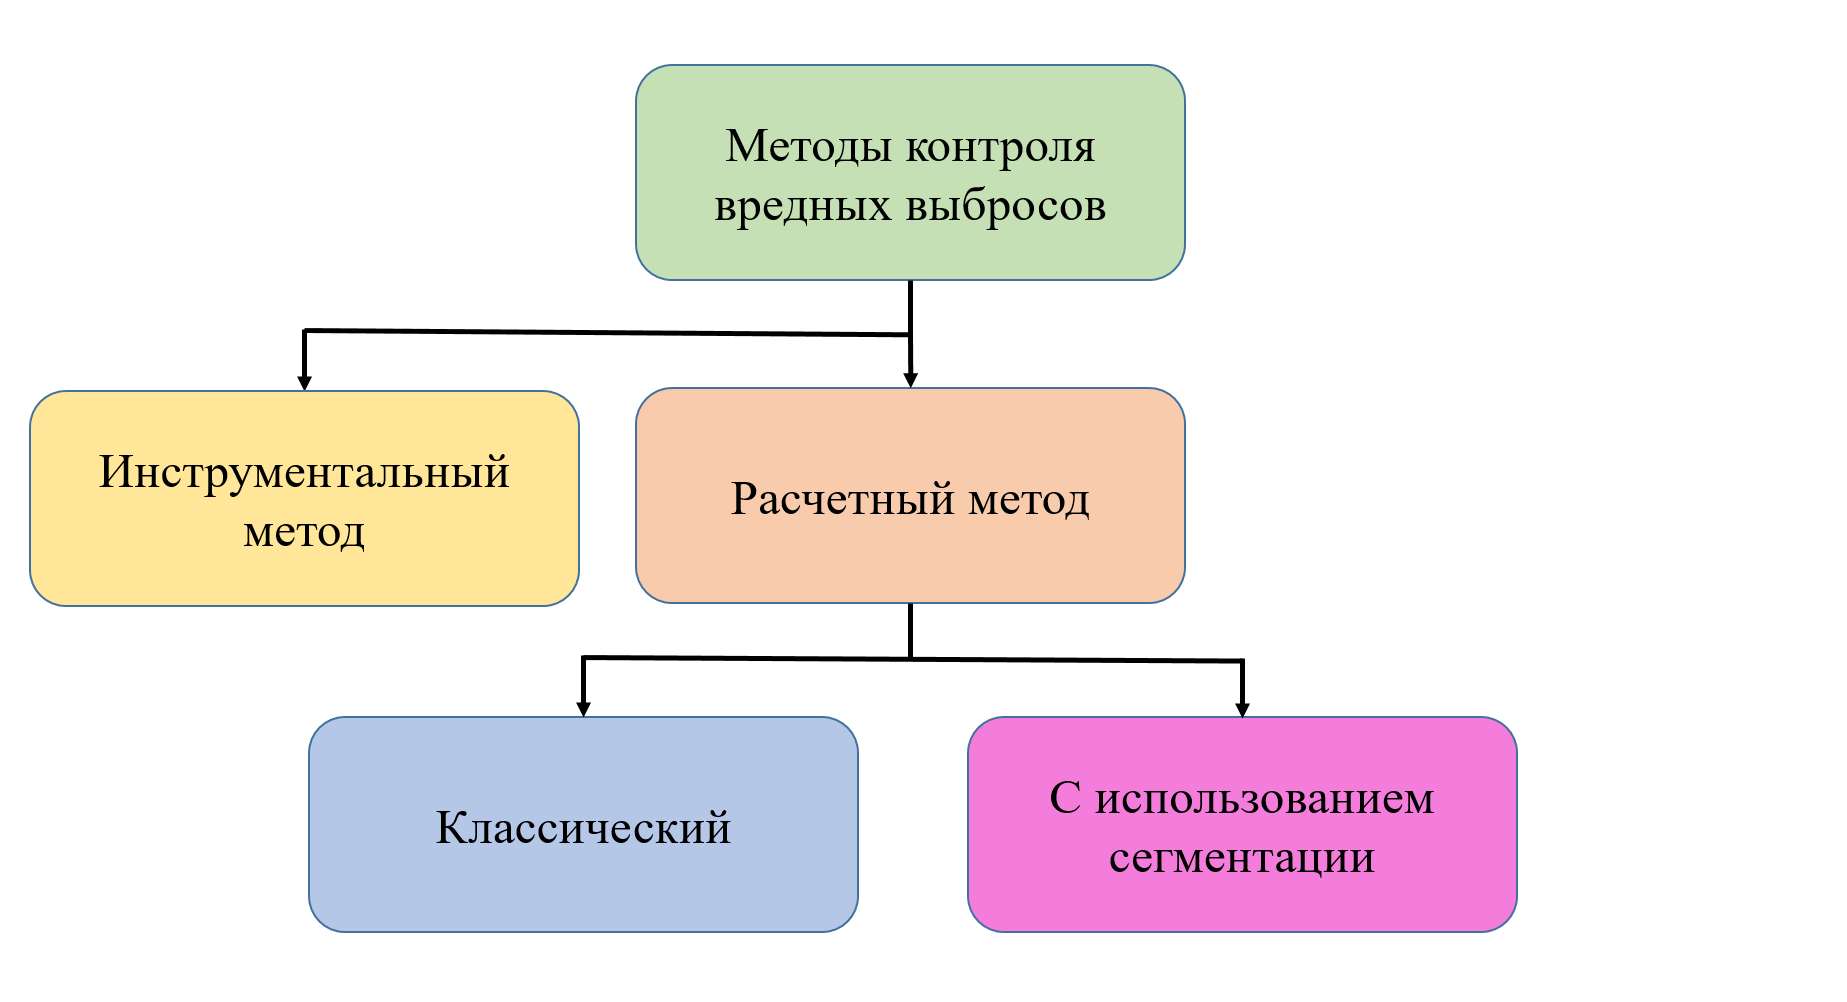
\includegraphics[width = \textwidth]{image/scheme1}	
		\end{figure}
	\end{frame}

	\begin{frame}
		\frametitle{Преемущества тепловизоров}
		\begin{enumerate}
			\justifying
			\item большая дешевизна;
			\item относительно высокая точность.
		\end{enumerate}
		\begin{figure}[ht!]
			\begin{subfigure}{.4\textwidth}
				\centering
				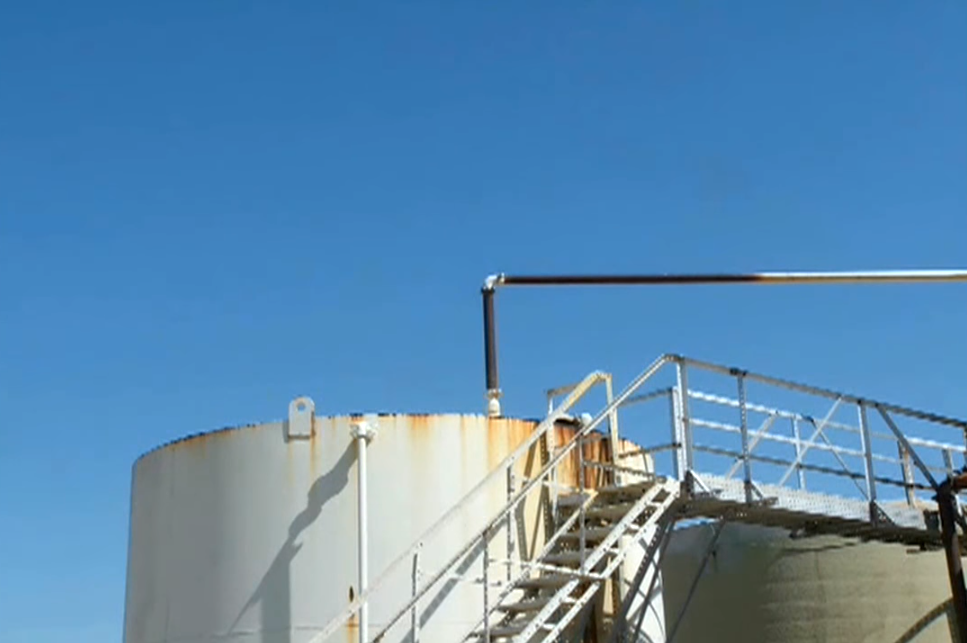
\includegraphics[width = \textwidth]{image/optic_invis}
				\caption{}
			\end{subfigure}
			\begin{subfigure}{.4\textwidth}
				\centering
				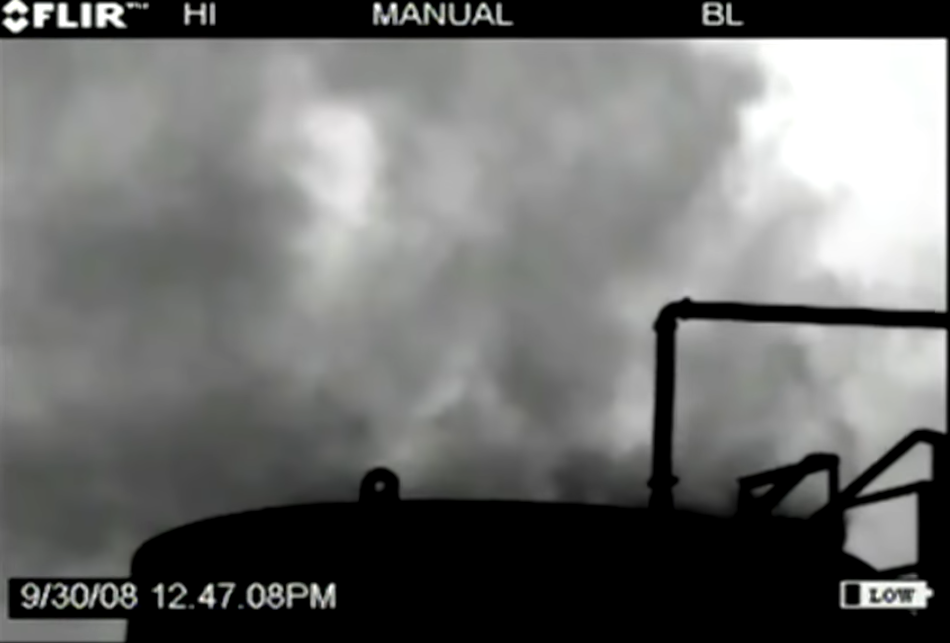
\includegraphics[width = \textwidth]{image/tep_vis}
				\caption{}
			\end{subfigure}
			\centering
			\caption{Преемущество перед сегментацией оптических снимков, где (a) оптическое изображение; (б) тепловизионное}
			\label{fig:Examples}
		\end{figure}
	\end{frame}

\section{Задача}

	\begin{frame}
		\frametitle{\insertsection} 
		\vspace*{-0.3cm}
		Необходимо востановить целевую функцию
		\begin{equation}
			f: X \rightarrow Z,
			\label{eq:segment_func}
		\end{equation}
	где $X$ -- пространство пар из RGB изображений и матриц температур;
	$Z$ - пространство масок где каждый элемент -- принадлежность пикселя дыму.
	\begin{figure}[ht!]
		\begin{subfigure}{.25\textwidth}
			\centering
			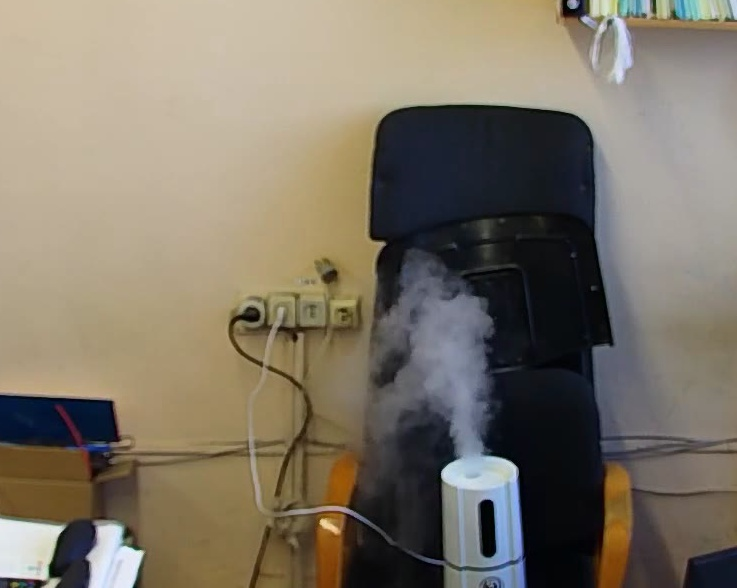
\includegraphics[width = \textwidth]{image/opt_examp}
			\caption{}
		\end{subfigure}
		\begin{subfigure}{.25\textwidth}
			\centering
			
\includegraphics[width = \textwidth]{image/tep_examp}
			\caption{}
		\end{subfigure}
		\begin{subfigure}{.25\textwidth}
			\centering
			
\includegraphics[width = \textwidth]{image/mask}
			\caption{}
		\end{subfigure}
		\centering
		\caption{Примеры полученых изображений, где (a) RGB изображение;(б) матрица температур; (г) полученная маска}
		\label{fig:Examples}
	\end{figure}
	\end{frame}

\section{Подготовка данных}

	\begin{frame}
		\frametitle{\insertsection} 
		\vspace{1cm}
		\begin{figure}
			\centering
			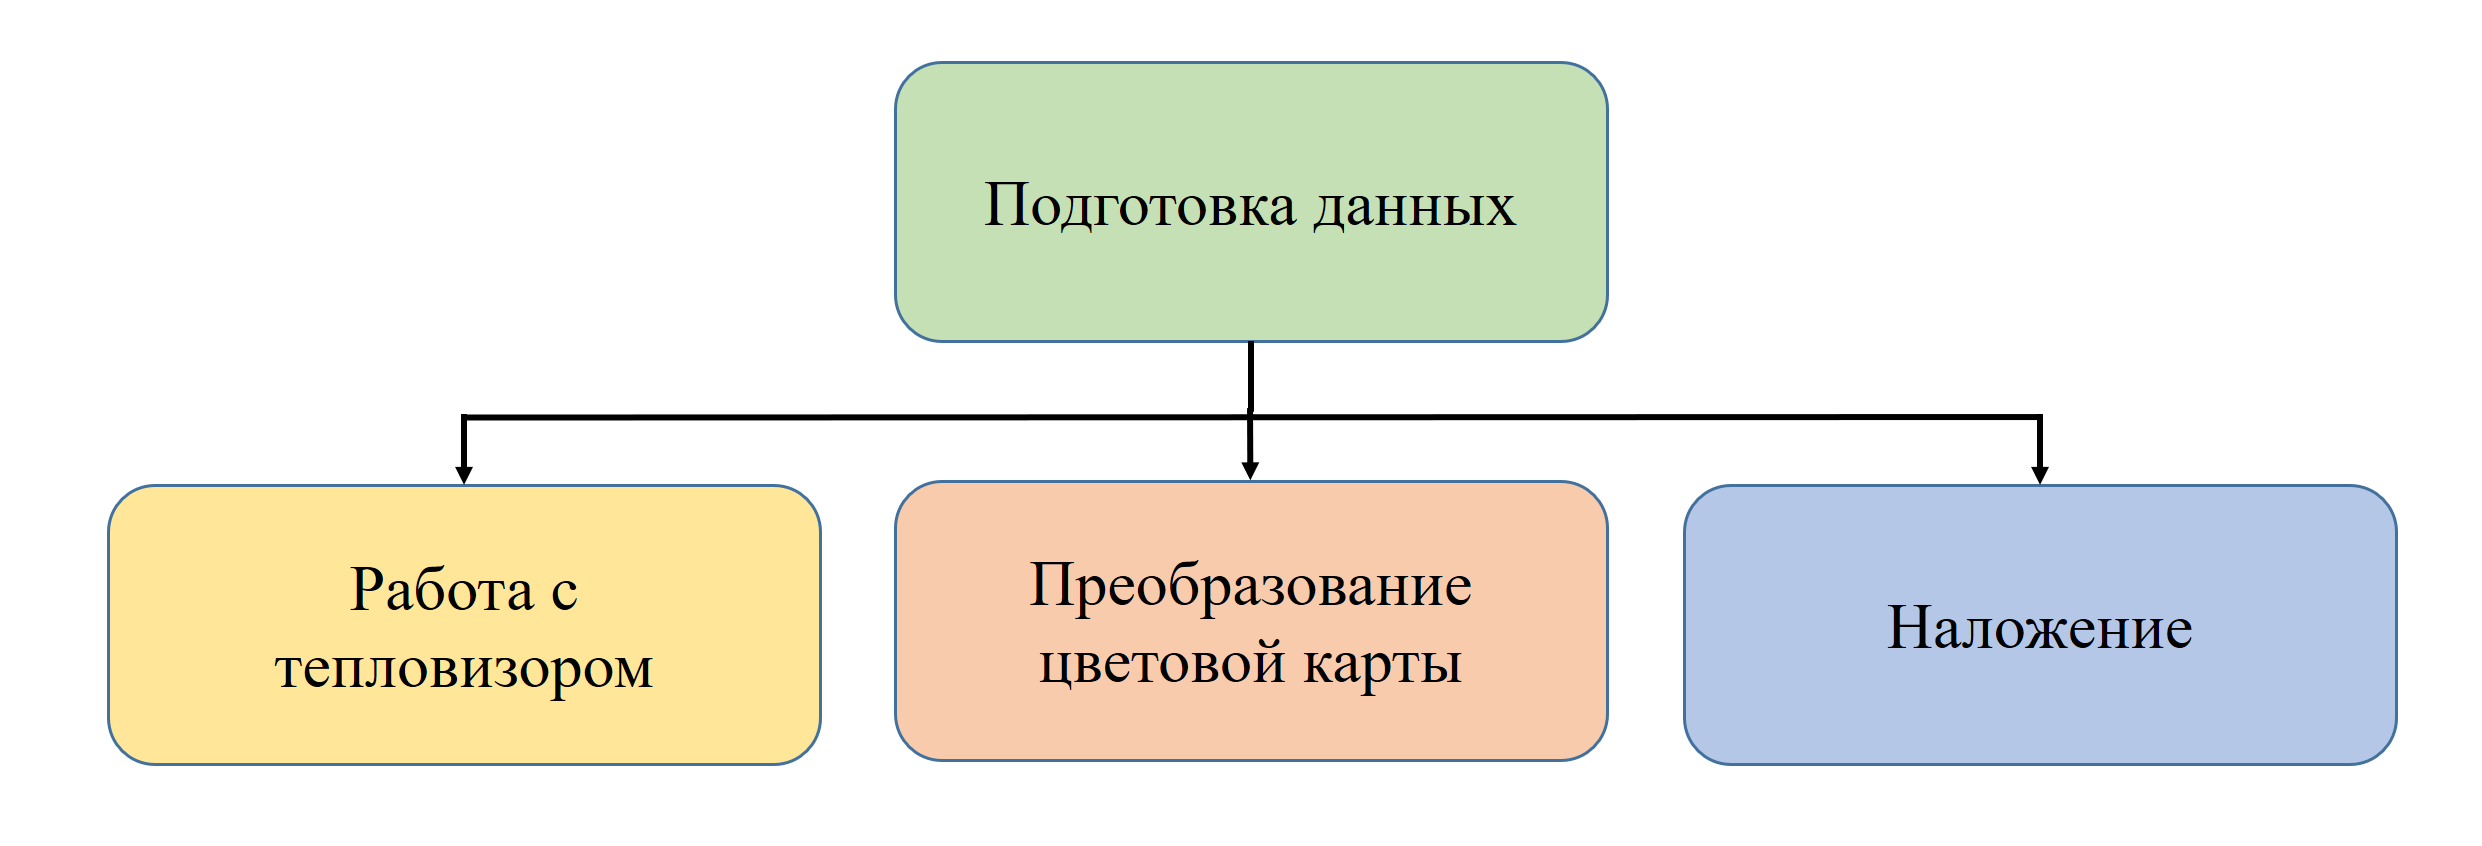
\includegraphics[width = \textwidth]{image/scheme2}	
		\end{figure}
	\end{frame}

	\begin{frame}
		\frametitle{Работа с тепловизором}
		\vspace{1cm}
		\begin{figure}[ht!]
			\begin{subfigure}{0.5\textwidth}
				\centering
				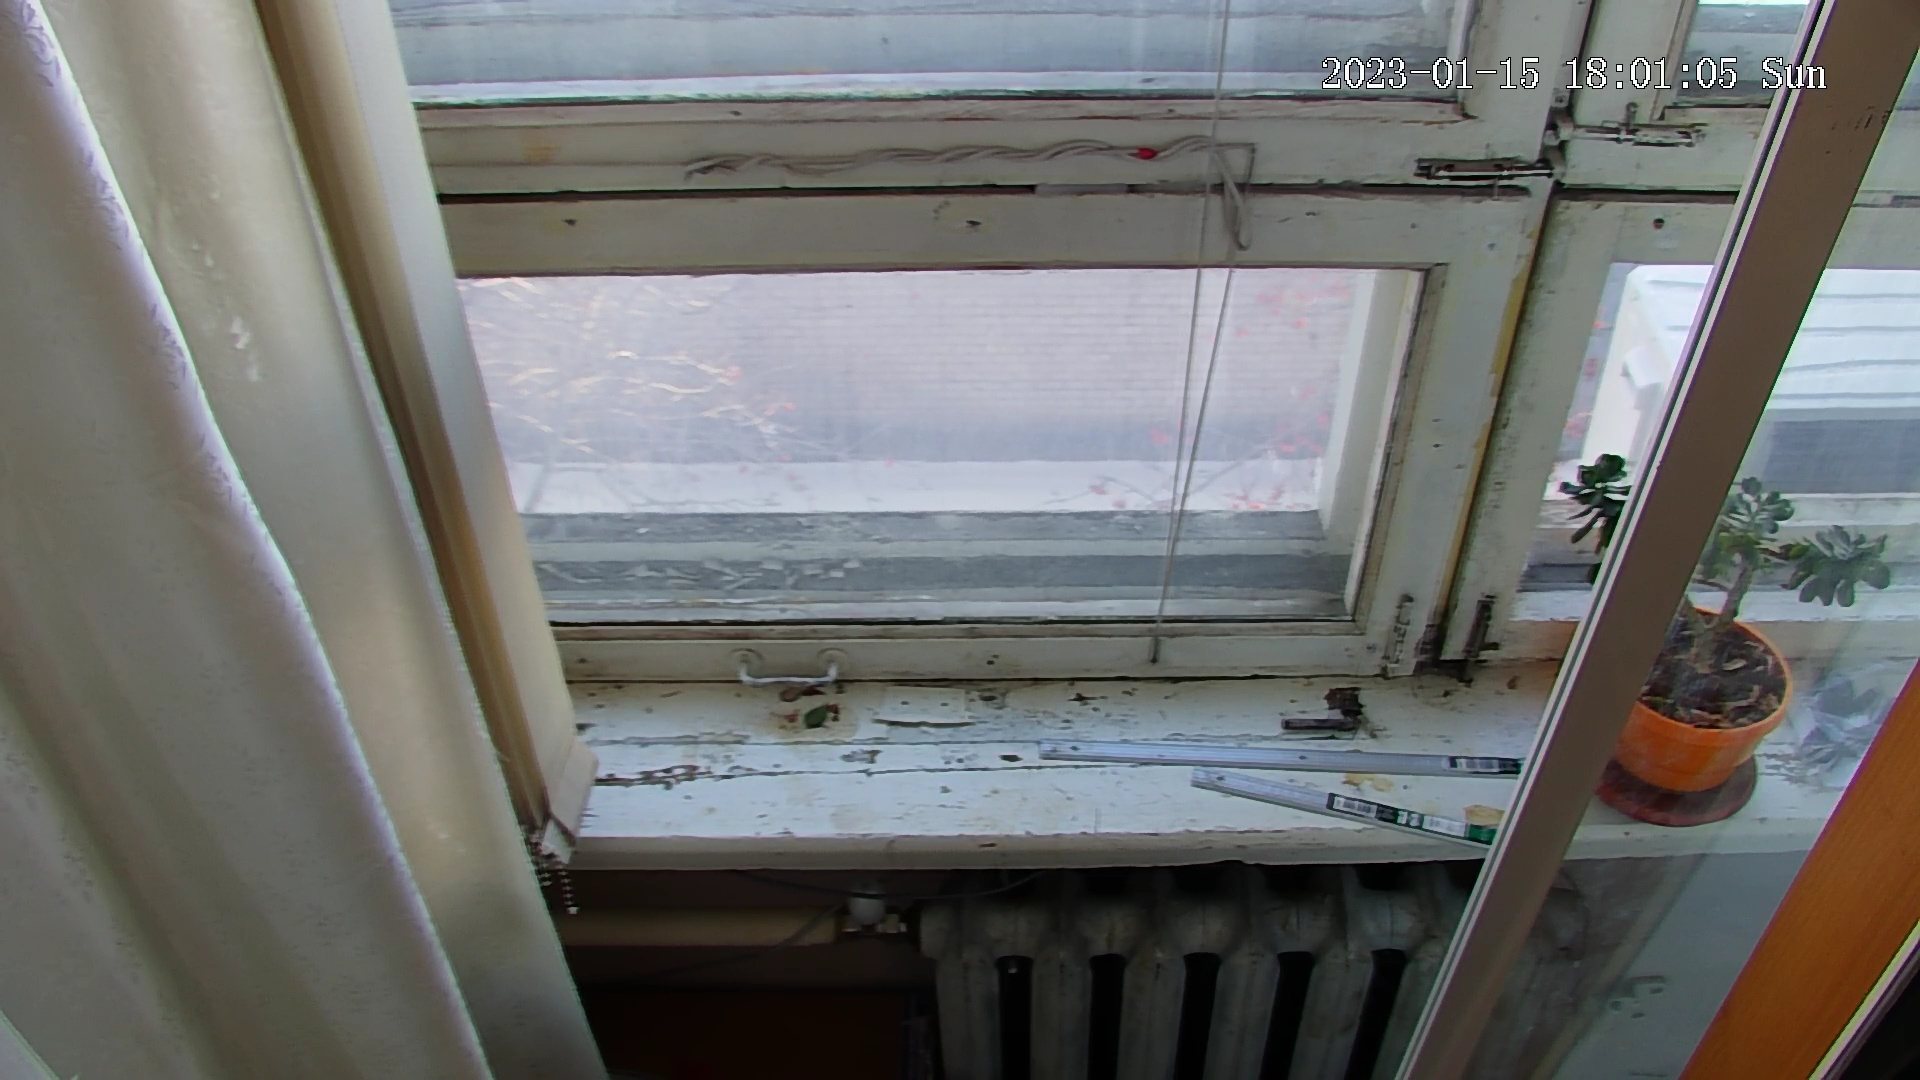
\includegraphics[width = \textwidth]{image/chapter_2/opt_example}
				\caption{}
			\end{subfigure}
			\begin{subfigure}{0.3\textwidth}
				\centering
				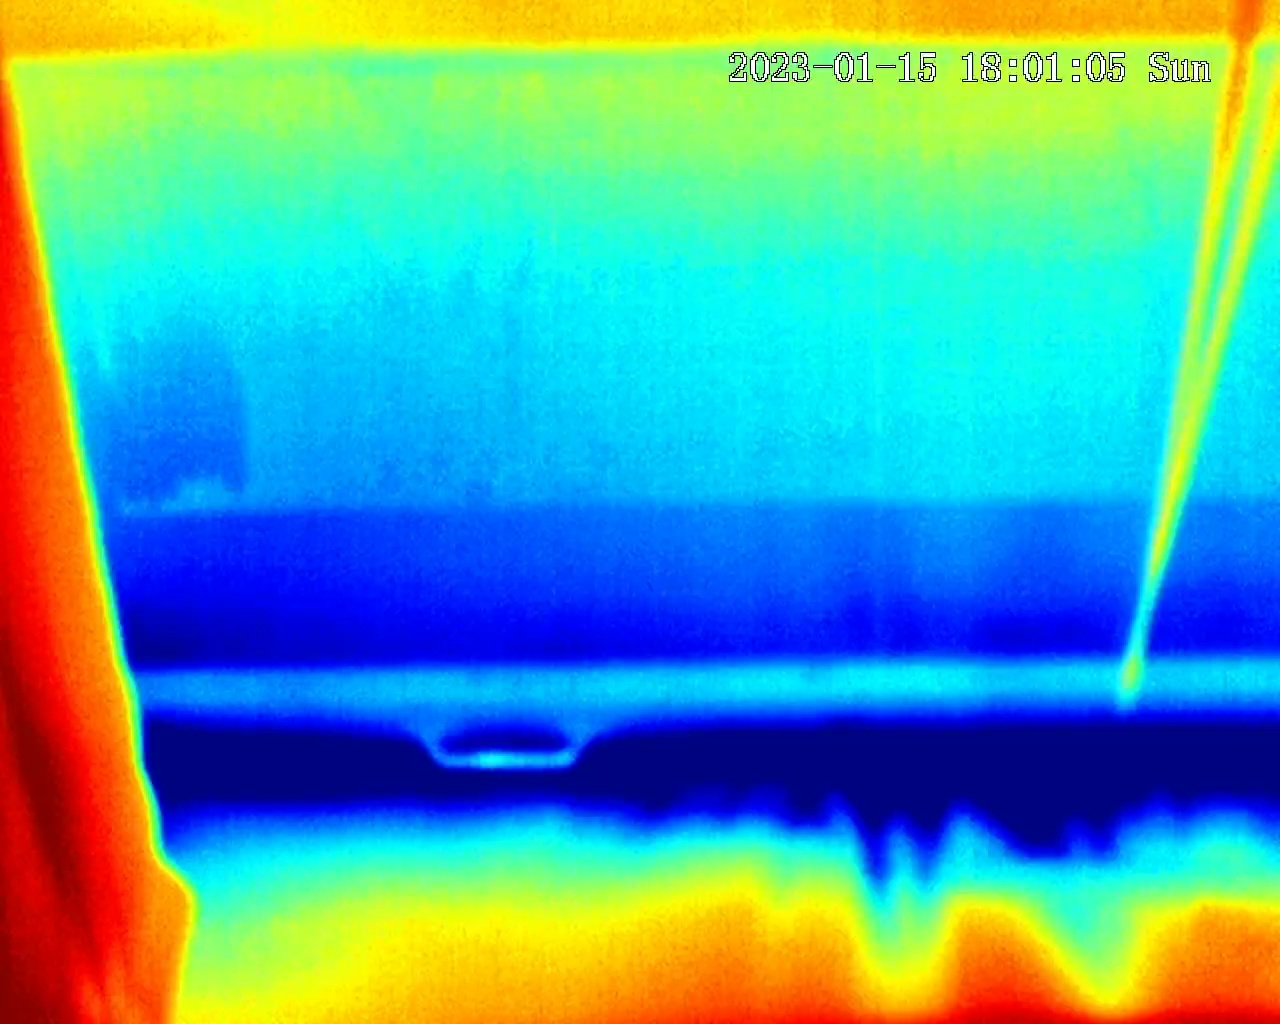
\includegraphics[width = \textwidth]{image/chapter_2/tep_example}
				\caption{}
			\end{subfigure}
			\centering
			\caption{Примеры полученых изображений, где \\(a) оптический снимок; (б) тепловой снимок}
			\label{fig:Examples}
		\end{figure}
	\end{frame}

	\begin{frame}
		\frametitle{Работа с тепловизором}
		\vspace*{-0.45cm}
		\begin{figure}[h!]
			\centering
			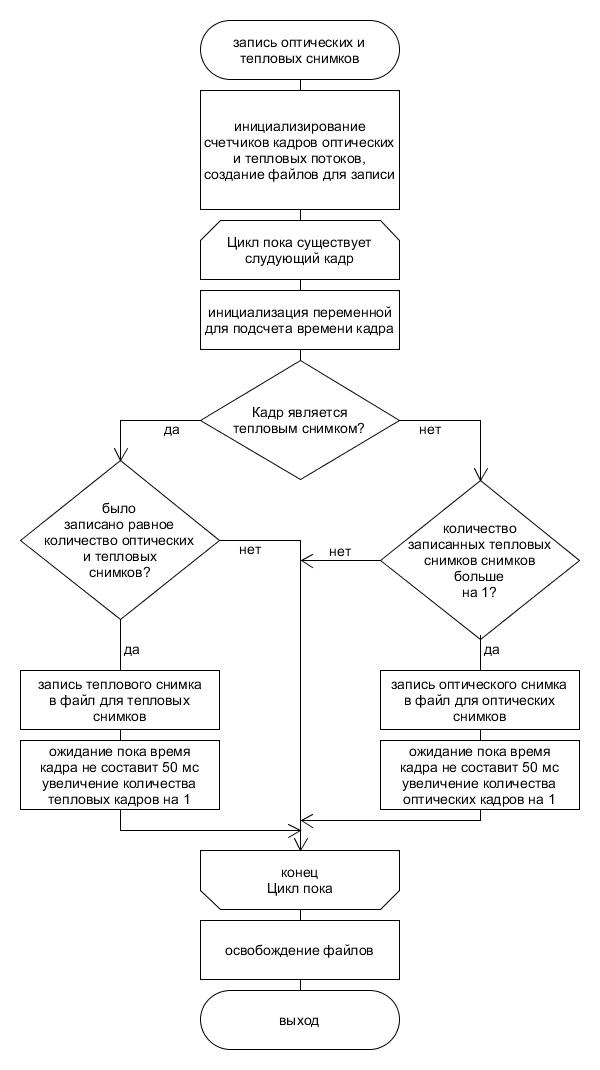
\includegraphics[width = \textwidth]{image/chapter_2/loaddata}	
			\caption{Алгоритм сохранения снимков}
			\label{fig:loaddata}
		\end{figure}
	\end{frame}

	\begin{frame}
		\frametitle{Преобразование цветовой карты}
		\vspace*{0.45cm}
		\begin{figure}[ht!]
			\begin{subfigure}{.45\textwidth}
				\centering
				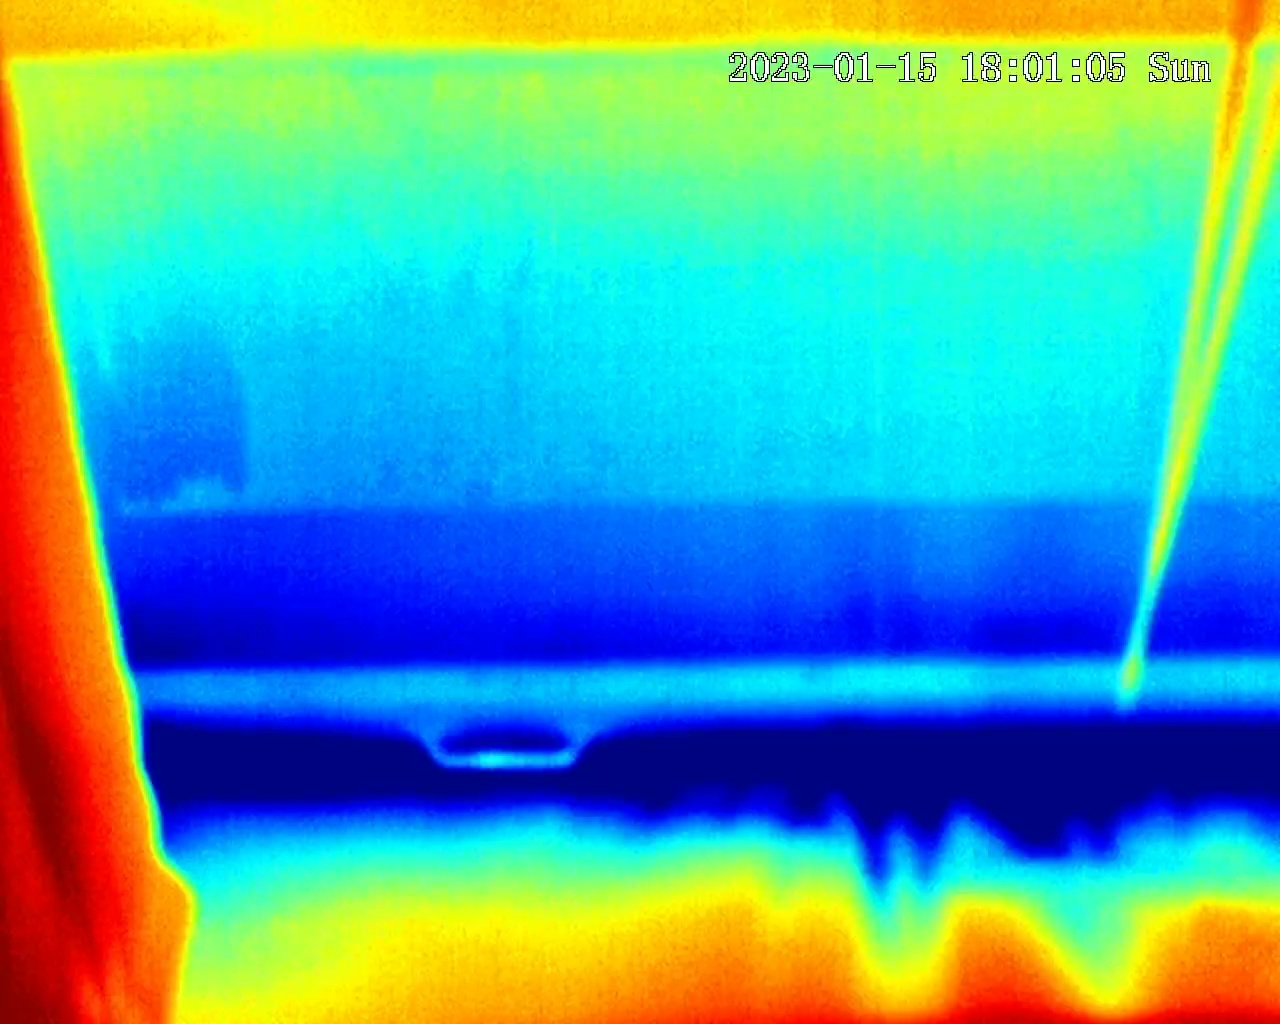
\includegraphics[width = 4cm]{image/chapter_2/tep_example}
				\caption{}
			\end{subfigure}
			\begin{subfigure}{.45\textwidth}
				\centering
				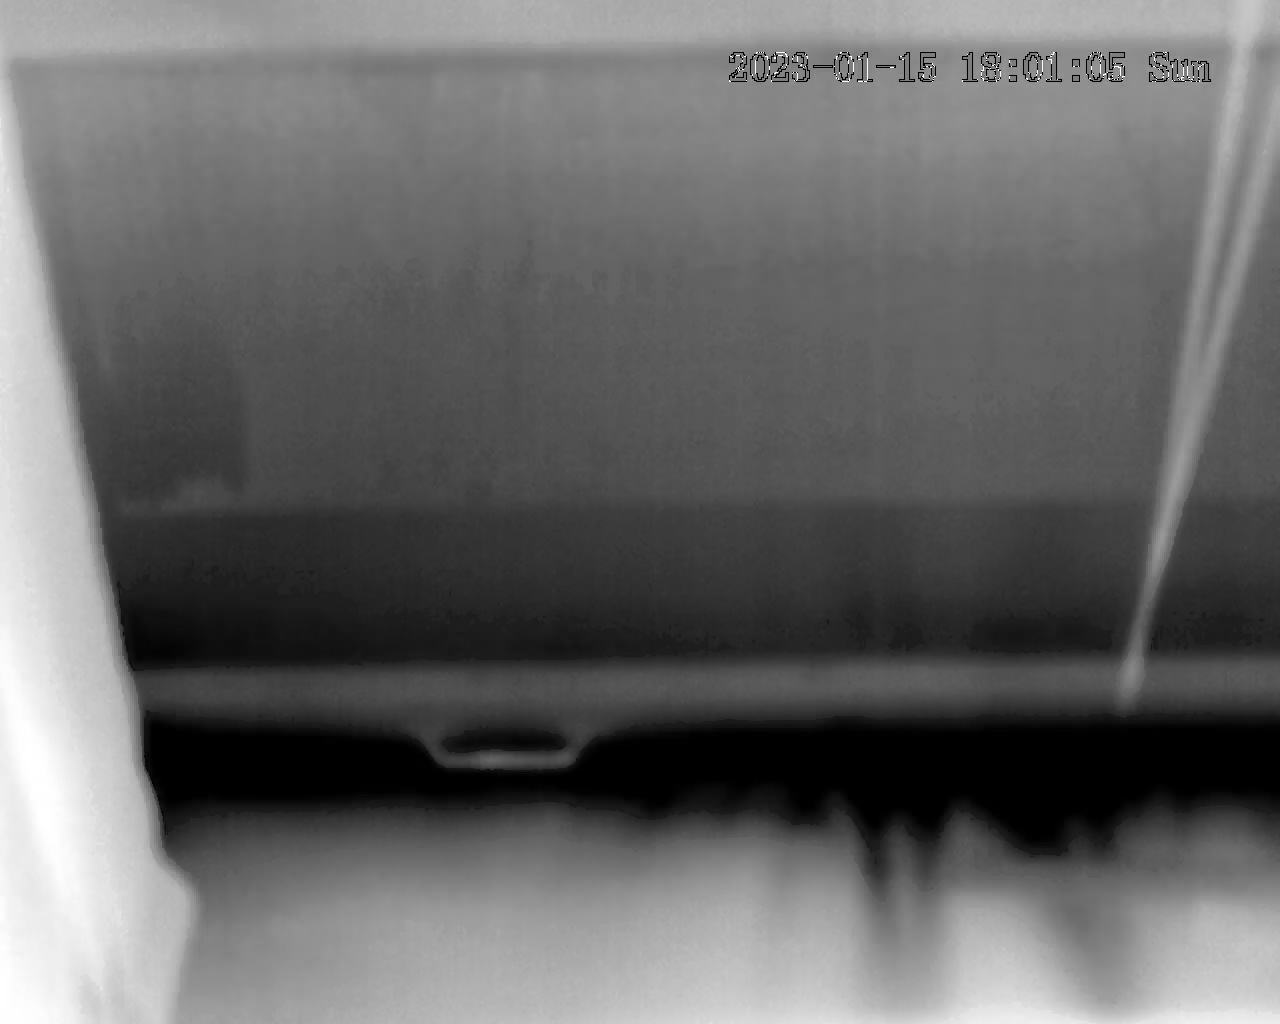
\includegraphics[width = 4cm]{image/chapter_2/gray_tep_example}
				\caption{}
			\end{subfigure}
			\centering
			\caption{Примеры преобразования цветовой карты, где\\ (a) до; (б) после}
			\label{fig:ResKNN}
		\end{figure}
	\end{frame}

	\begin{frame}
		\frametitle{Модель <<FlannBasedMatcher>>}
		
		Эта модель решает задачу классификации и работает на основе метода $k$-ближайших соседей, оптированного с помощью структуры данных <<$k$-мерное дерево>>.
		\begin{figure}[h!]
			\centering
			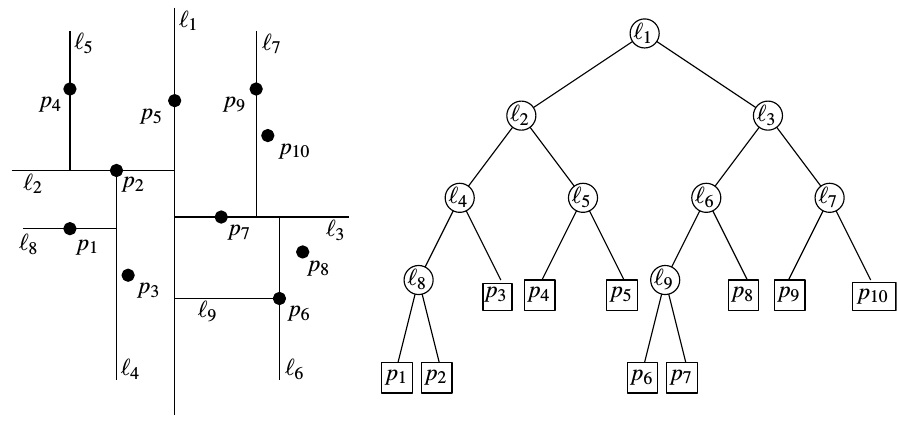
\includegraphics[width = 6cm]{image/chapter_2/kdtreeexample}	
			\caption{Пример построения k-мерного дерева}
			\label{fig:kdtreeexample}
		\end{figure}
	\end{frame}
	
	\begin{frame}
		\vspace*{-0.35cm}
		\begin{figure}[ht!]
			\begin{subfigure}{.47\textwidth}
				\centering
				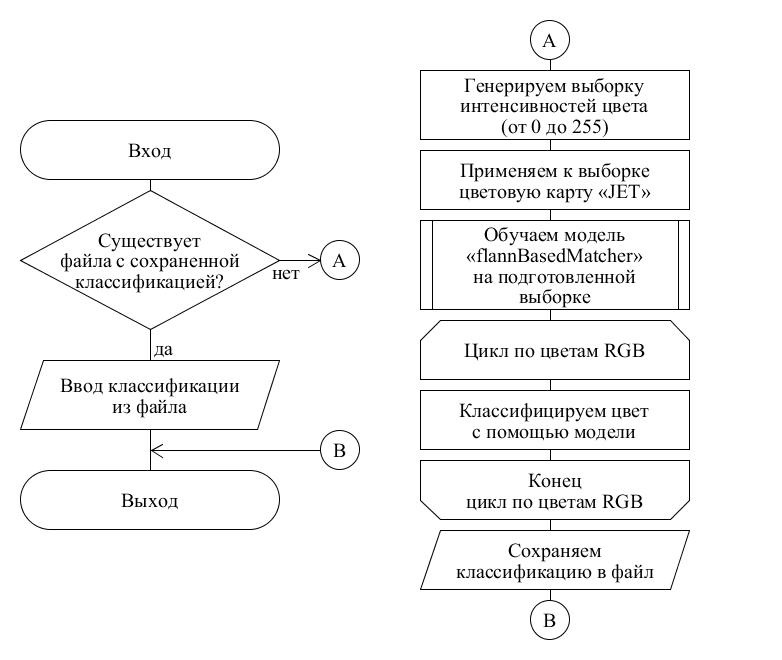
\includegraphics[width = \textwidth]{image/chapter_2/colorclassification}
				\caption{}
			\end{subfigure}
			\begin{subfigure}{.21\textwidth}
				\centering
				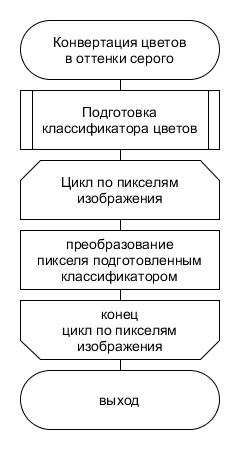
\includegraphics[width = \textwidth]{image/chapter_2/colorclassification2}
				\caption{}
			\end{subfigure}
			\centering
			\caption{Алгоритмы преобразования цветов, где (а) алгоритм подготовки классификатора цветов; (б) алгоритм преобразования}
			\label{fig:Examples}
		\end{figure}
		
	\end{frame}

	\begin{frame}
		\frametitle{Метрика точности преобразования цветов}
%		\vspace*{0.2cm}
		\begin{equation}
			Acc = 1 - \frac{\sum\limits_{i=1}^h \sum\limits_{j=1}^w |P^{true}_{ij} - P^{conv}_{ij}|}{255wh},
			\label{eq:flanaccuracy}	
			\vspace*{0.2cm}
		\end{equation}
		где $w$ -- высота кадра;\\ \hfill \break
		$h$ -- размеры кадра;\\ \hfill \break
		$P^{true}$ -- некоторое изображение в оттенках серого;\\ \hfill \break
		$P^{conv}$ -- то же самое изображение, но с наложеной цветовой картой, сжатое с помощью JPEG и обработанное алгоритмом преобразования. 
	\end{frame}

	\begin{frame}
		\frametitle{Метрика точности преобразования цветов}
		\vspace*{-0.35cm}
		\begin{figure}[h!]
			\centering
			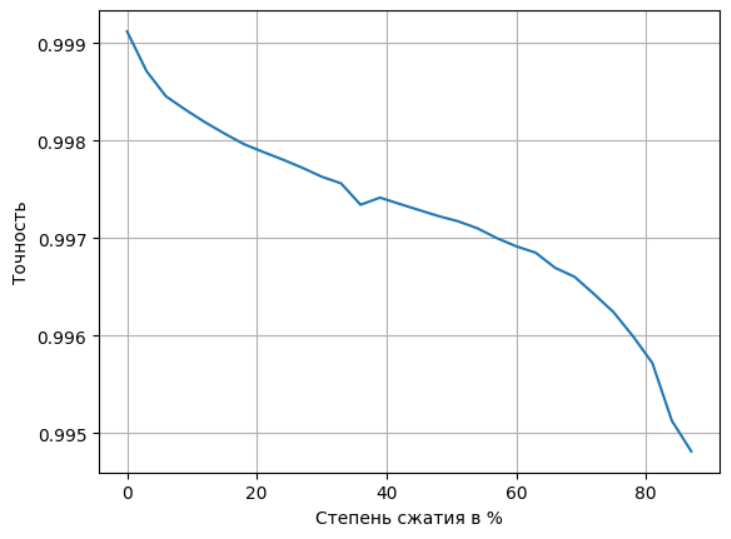
\includegraphics[width = 0.8\textwidth]{image/accuracy_plot}	
			\caption{Зависимость точности от степени сжатия}
			\label{fig:fullprepare}
		\end{figure}
	
	\end{frame}

	\begin{frame}
		
		\begin{figure}[h!]
			\centering
			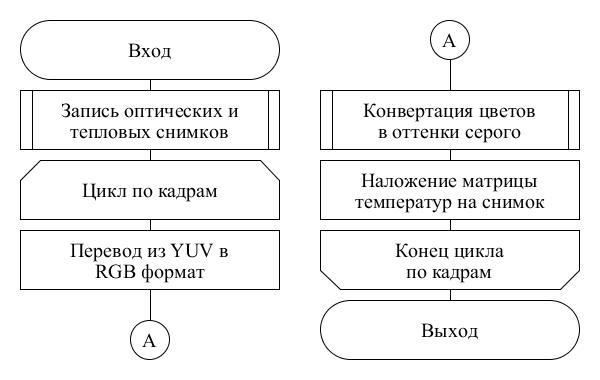
\includegraphics[width = 0.23\textwidth]{image/chapter_2/fullprepare}	
			\caption{Алгоритм подготовки данных}
			\label{fig:fullprepare}
		\end{figure}
		
	\end{frame}

\section{Результаты}

	\begin{frame}
		\frametitle{Результаты}
		\vspace*{0.65cm}
		\begin{figure}[ht!]
			\begin{subfigure}{.30\textwidth}
				\centering
				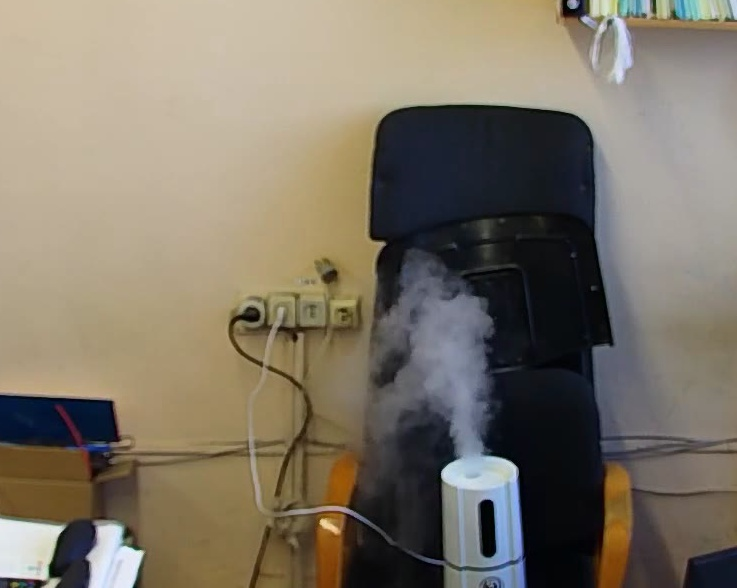
\includegraphics[width = \textwidth]{image/opt_examp}
				\caption{}
			\end{subfigure}
			\begin{subfigure}{.30\textwidth}
				\centering
				
\includegraphics[width = \textwidth]{image/tep_examp}
				\caption{}
			\end{subfigure}
			\begin{subfigure}{.30\textwidth}
				\centering
				
\includegraphics[width = \textwidth]{image/mask}
				\caption{}
			\end{subfigure}
			\centering
			\caption{Примеры полученых изображений, где (a) RGB изображение; (б) матрица температур; (г) полученная маска}
			\label{fig:Examples}
		\end{figure}
	\end{frame}

\end{document}
